%---------------------------------------------------------------------------
\svnidlong 
{$HeadURL: https://svn.fil.univ-lille1.fr/svn/sedoglav_PDC/trunk/Cours/09/09.tex $} 
{$LastChangedDate: 2013-02-12 16:26:32 +0100 (Tue, 12 Feb 2013) $} 
{$LastChangedRevision: 86 $} 
{$LastChangedBy: sedoglav $} 
\svnid{$Id: 09.tex 86 2013-02-12 15:26:32Z sedoglav $} 
%------------------------------------------------------------------------------
%\section{Prol\'egon\`emes}
%\label{sec:Prolegomenes}
%------------------------------------------------------------------------------
%\begin{slide}
%  \listofslides
%\begin{slide}%  \slideheading{Plan de la s\'eance}%
%  \begin{enumerate}
%  \item Les classes d'allocation des variables en~C
%%  \item Une technique virale~: le d\'ebordement de pile
%  \item Deux cons\'equences du passage de param\`etres par la pile
%  \item D\'efinition~: un contexte dans la pile d'ex\'ecution (stack frame)
%  \item Quelques exemples de passage de param\`etres (point de vue assembleur)
%  \item Quelques exemples de passage de param\`etres (point de vue~C)
%  \end{enumerate}    
%\end{slide}
%------------------------------------------------------------------------------
  \section{Les classes d'allocation des variables}%
\begin{frame}
  \frametitle{Les classes d'allocation des variables}%
 En~C, les variables ont pour attribut~:
  \begin{itemize}
  \item leur nom~: un identificateur~;
  \item leur type~: type de base ou d\'efini par l'utilisateur~;
  \item une classe d'allocation indiquant~: 
    \begin{itemize}
    \item le type de l'emplacement m\'emoire o\`u est allou\'ee la variable~;
    \item sa dur\'ee de vie~;
    \item sa visibilit\'e par les diff\'erentes fonctions.
    \end{itemize}
  \end{itemize}
  \par\bigskip
  Il y a~$5$ classes d'allocation~:
  \par
  \begin{center}
    \begin{tabular}{ccccc}
      externe & automatique & statique & ``register'' & volatile
    \end{tabular}
  \end{center}
\end{frame}
%------------------------------------------------------------------------------
\begin{frame}
  Les variables externes ({\tt extern}) sont~: 
  \begin{itemize}
  \item allou\'ees en zone statique de donn\'ees (dans un segment de
    donn\'ees)~;
  \item allou\'ees \`a la compilation (valeur par d\'efaut~0)~;
  \item dur\'ee de vie du processus~;
  \item visibles depuis toutes les fonctions.
  \end{itemize}
  \par\bigskip
  Les variables statiques ({\tt static}) sont~:
  \begin{itemize}
  \item allou\'ees comme les variables externes~;
  \item et si elles sont d\'efinies~:
    \begin{itemize}
    \item \`a l'ext\'erieur de toute fonction, elles sont visibles
      depuis les fonctions d\'eclar\'ees dans le fichier source les
      contenant~;
    \item \`a l'int\'erieur d'une fonction, elles sont visibles
      depuis la fonction seulement, mais reste allou\'ees en dehors de
      l'ex\'ecution de la fonction (valeur conserv\'ee entre les diff\'erents appels).
    \end{itemize}
  \end{itemize}
\end{frame}
%------------------------------------------------------------------------------
\begin{frame}
  Les variables automatiques ({\tt auto}) sont~:
  \begin{itemize}
  \item allou\'ees dynamiquement sur la pile (valeur initiale
    ind\'etermin\'ee)~;
  \item allou\'ees \`a chaque entr\'ee dans la fonction ou le bloc
    o\`u la variable est d\'efinie (param\`etres, variables
    locales)~;
  \item dur\'ee de vie de la fonction ou du bloc~;
  \item visibles uniquement depuis la fonction ou le bloc.
  \end{itemize}
  \par\bigskip
  Les variables de registres ({\tt register}) sont~: 
  \begin{itemize}
  \item allou\'ees si possible dans un
    registre du processeur~;
  \item des variables de type simple uniquement~;
  \item des variables de classe automatique uniquement~;
  \item et ne poss\`edent pas d'adresse.
  \end{itemize}
\end{frame}
%------------------------------------------------------------------------------
\begin{frame}[fragile]
  Par exemple, on peut avoir le code suivant~:
\begin{verbatim}
   int global = 1; /* d\'efinition d'une variable 
                      externe (globale)          */
                                    
   extern int extern_global ; /* d\'eclaration d'une variable
                      globale d'un autre fichier (externe) */

   static int global_privee = 2 ; /* globale au fichier,
             invisible depuis d'autres fichiers (statique) */
   int
   fonction(int param) {/* param\`etre (automatique)    */
    auto int local = 3 ;  /* variable automatique (locale) */
                      /* le mot clef auto ne sert \`a rien */
    static int local_static = 4 ; /* variable 
       statique (locale) valeur inchang\'ee entre 2 appels */

    register int i = 5 ;     /* variable register (locale) */

    return i++ ;
  }
\end{verbatim}
\end{frame}
%------------------------------------------------------------------------------
\begin{frame}[fragile]
Le code assembleur correspondant est~:
\begin{verbatim}
int global = 1;                          .data                
                                 .globl global                   
extern int extern_global ;       global:                      
                                         .long   1            
static int global_privee = 2 ;   global_privee:               
                                         .long   2            
int fonction(int param) {        local_static.0:              
   int local = 3 ;                       .long   4            
                                         .text                
   static int local_static = 4 ; .globl fonction              
                                 fonction:                    
   register int i = 5 ;                pushl   %ebp         
                                       movl    %esp, %ebp   
   return i++ ;                        subl    $4, %esp     
}                                      movl    $3, -4(%ebp) 
                                       movl    $5, %eax     
                                       leave                
                                       ret                  
\end{verbatim}
\end{frame}
%------------------------------------------------------------------------------
\begin{frame}[fragile]
  \section{Effet des mots clef static et extern sur les fonctions}%
\begin{verbatim}
extern int ailleurs(int) ;              .text                    
                                        .type   foo,@function    
static int foo(void){            foo:                             
        return 1 ;                      pushl   %ebp             
}                                       movl    %esp, %ebp       
                                        movl    $1, %eax         
int bar(void){                          popl    %ebp             
        return 1 ;                      ret                      
}                               .Lfe1:                           
                                        .size   foo,.Lfe1-foo    
                                .globl bar                       
/* la fonction ailleurs                 .type   bar,@function    
   est d\'eclar\'ee mais        bar:                             
   d\'efinie dans un autre              pushl   %ebp             
   fichier source (i.e. object).        movl    %esp, %ebp       
                                        movl    $1, %eax         
   la fonction foo n'est pas            popl    %ebp             
   accessible depuis un autre           ret                      
   fichier alors que bar l'est.         .Lfe2:                           
                                */      .size   bar,.Lfe2-bar    
\end{verbatim}
\end{frame}
%------------------------------------------------------------------------------
\begin{frame}[fragile]
  Les variables \texttt{volatiles} sont susceptibles d'\^etre
  modifi\'ees ind\'ependamment du code les d\'eclarant. Consid\'erons
  l'exemple suivant (seul dans un fichier sources)~:
\begin{verbatim}
static int foo; /* foo pourrait \^etre un pointeur sur 
                   un segment de m\'emoire partag\'ee */
void 
bar(void){
   foo=0 ;
   while(foo!=1)
     continue ;
}
\end{verbatim}
  Un compilateur en optimisant ce code remplacera la boucle par
  \verb+while(1)+ car la classe d'allocation \texttt{static} lui
  assure que seule la fonction \texttt{bar} peut modifier
  \texttt{foo}. Cependant, l'emplacement m\'emoire associ\'e \`a la
  variable pourrait \^etre partag\'e --- et donc modifiable --- par un
  autre processus (voir l'unit\'e d'enseignement \emph{Pratique des
    syst\`emes}) et l'optimisation du compilateur ne pas correspondre
  \`a la volont\'e du programmeur.
\end{frame}
%-----------------------------------------------------------------------------
\begin{frame}[fragile]
  L'usage de la classe d'allocation \texttt{volatile} supprime
  l'optimisation concernant la variable ainsi qualifi\'ee. Le code~:
\begin{verbatim}
static volatile int foo;

void 
bar
(void)
{
   foo=0 ;
   while(foo!=1)
     continue ;
   return ;
}
\end{verbatim}
  correspond donc au cas de figure au la variable \texttt{foo} est
  partag\'ee (par exemple entre deux processus l\'egers ou dans un segment
  de m\'emoire partag\'e --- cf.\ cours Pratique des Syst\`emes).
  \par\medskip
  Sans \texttt{volatile}, le compilateur simplifie ce code en boucle infinie (comme
  \texttt{foo} n'est pas modifi\'e, cette variable est supprim\'ee).
\end{frame}
%------------------------------------------------------------------------------
\begin{frame}[fragile]
  Une variable dont le type est qualifi\'e par \verb+const+ ne peut pas \^etre modifi\'ee.
  \par\smallskip
  Ce qualificatif permet au programmeur de s'assurer de ne pas modifier des variables
  pass\'ees par r\'ef\'erence comme par dans le cas suivant~:
\begin{verbatim}
#include <string.h>
int strcmp(const char *, const char *);
\end{verbatim}
  Ainsi, on est sur que cette fonction ne va pas modifier les cha\^\i{}nes de caract\`eres
  pass\'ees en arguments.
  \par\smallskip
  Ce modificateur de type impose la d\'efinition au moment de la
  d\'eclaration (\verb+const int a=0;+ et pas \verb+const int a; a=0;+).
  \par\smallskip
  Remarquons que les qualificateurs de types peuvent \^etre utilis\'es finement~:
\begin{verbatim}
   const char c ;         /* caract\`ere constant */
   const char *s ; /* pointeur vers caract\`eres constants */
   char const *s ; /* pointeur constant vers caract\`eres */
   const char * const s ; /* pointeur constant 
                             vers caract\`eres constants */
\end{verbatim}

\end{frame}
%-----------------------------------------------------------------------------
\begin{frame}[fragile]
  \section{Ordre d'\'evaluation des param\`etres}%
  Attention aux surprises lors de l'\'evaluation des param\`etres \`a
  transmettre~:
\begin{verbatim}
#include <stdio.h>        .rodata 
                    .LC0: .string "le premier argument %c..."    
int main(void){           .text .globl main        
                              main:   pushl   %ebp  
   int foo = 'a' ;                    movl    %esp, %ebp 
                                      subl    $8, %esp        
   printf("le premier argument %c     movl    $97, -4(%ebp)   
      et le second %c\n",foo,foo++);  subl    $4, %esp 
   return 0 ;                         movl    -4(%ebp), %eax 
}                                     pushl   %eax             
                                      leal    -4(%ebp), %eax 
$ a.out                               incl    (%eax)         
le premier argument b et le second a  pushl   -4(%ebp)  
                                      pushl   $.LC0    
                                      call    printf       
                                      addl    $16, %esp         
                                      movl    $0, %eax 
                                      leave ret     
\end{verbatim}
\end{frame}
%------------------------------------------------------------------------------
\begin{frame}[fragile]
  \section{Fonction \`a nombre variable de param\`etres}%
  Il est possible de d\'eclarer une fonction comme ayant un nombre
  variable de param\`etres en \og d\'eclarant \fg\ les param\`etres optionnels
  par l'unit\'e lexicale \ldots\ (3 points \`a la suite)~:
\begin{verbatim}
int 
foo
(char *par_obl, ...)
{
   return 0 ;
}
\end{verbatim}
  Une fonction peut avoir \`a la fois des param\`etres obligatoires et des
  param\`etres optionnels, les param\`etres obligatoires apparaissant en
  premier et l'unit\'e lexicale ... apparaissant en derni\`ere position
  dans la liste de d\'eclaration des param\`etres formels.
  \par
  G\'en\'eralement, un param\`etre obligatoire indique le nombre et le
  type des param\`etres optionnels comme dans le cas de printf~:
\begin{verbatim}
printf("premier argument %c et second %c\n",foo,foo++) ;
\end{verbatim}
\end{frame}
%------------------------------------------------------------------------------
\begin{frame}[fragile]
  \frametitle{Un exemple d'utilisation (param\`etres optionnels de m\^eme type)}
\begin{verbatim}
int somme(int nbpar, ...){
  int *pt = &nbpar ; /* on fait pointer pt 
                        sur le premier param\`etre */
  int res = 0; 

  for(;nbpar>0;nbpar--){
      pt++       ; /* on passe au param\`etre suivant */
      res += *pt ;
    }
  return res ;
}

int 
main(void){
  return somme(3,1,2,3)+somme(4,4,5,3,1) ;
}
\end{verbatim}
\end{frame}
%------------------------------------------------------------------------------
\begin{frame}[fragile]
  \section{ D\'efinition~: un contexte dans la pile d'ex\'ecution (stack frame)}%
  On appelle contexte d'un appel de fonction dans la pile d'ex\'ecution la
  partie de la pile associ\'ee~:
  \begin{itemize}
  \item param\`etres d'appels~;
  \item adresse de retour et ancien pointeur de contexte \%\textsc{ebp}~;
  \item variables automatiques de la fonction.
  \end{itemize}
  \par
  Les diff\'erentes portions de pile correspondant aux diff\'erents
  contextes d'ex\'ecution peuvent \^etre obtenues dans gdb par~:
  \begin{itemize}
  \item backtrace~: les contextes disponibles
\begin{verbatim}
(gdb) backtrace
#0  traduction (code=0xbffff660 "oeu") at SMS.c:12
#1  0x08048532 in main () at SMS.c:45
#2  0x400327f7 in __libc_start_main
\end{verbatim}
  \item info frame nb~: qui affiche un contexte
\begin{verbatim}
(gdb) info frame 2
Stack frame at 0xbffff6f8: eip = 0x400327f7 in _main; 
saved eip 0x8048301 caller of frame at 0xbffff6d8  
Arglist at 0xbffff6f8, args: 
Locals at 0xbffff6f8, Previous frame's sp in esp
 Saved registers: ebp at 0xbffff6f8, eip at 0xbffff6fc
\end{verbatim}
  \end{itemize}
\end{frame}
%------------------------------------------------------------------------------
\section{setjmp/longjmp}
%------------------------------------------------------------------------------
\begin{frame}[fragile]
  On peut \'etendre la notion de contexte en y associant en plus des informations concernant 
  la pile d'ex\'ecution, l'\'etat des registres du  processeur (\%\textsc{eax}, \%\textsc{eip}, \%\textsc{cs}, etc).
  \par\medskip
  Ce faisant, on peut faire des branchements non-locaux (i.e.\ des branchements \`a un endroit
  presque arbitraire du code) sans utiliser \verb+goto+. Deux fonctions de la librairie standard sont d\'edi\'ees
  \`a cet effet. Sch\'ematiquement,
  \begin{itemize}
  \item \texttt{setjmp} m\'emorise son contexte juste avant son \textsc{ret}~;
  \item \texttt{longjmp} permet de r\'etablir le contexte m\'emoris\'e en pla\c{c}ant
	son second argument dans \%\textsc{eax}.
  \end{itemize}
\begin{verbatim}
#include <setjmp.h>
#include <stdio.h>
int main (void){
jmp_buf env;
int i = setjmp(env) ; /* au premier appel setjmp retourne 0 */
printf("i = %d\n",i);
if(i == 2) return 0 ;
longjmp(env,2) ; /* on branche sur setjmp qui retourne 2 */
return 1 ; /* cette instruction n'est jamais ex\'ecut\'ee */
}
\end{verbatim}
\end{frame}
%------------------------------------------------------------------------------
\begin{frame}[fragile]
  Dans l'exemple pr\'ec\'edent, \texttt{setjmp} et  \texttt{longjmp} sont utilis\'ees dans la
  m\^eme fonction mais g\'en\'eralement, ces fonctions sont utilis\'ees pour la gestion 
  d'erreurs et la programmation des syst\`emes (signal).
  \par\smallskip\textbf{Limitation~:} 
  \texttt{longjmp} ne permet pas de revenir \`a n'importe quel point m\'emoris\'e par l'appel \texttt{setjmp}~; ce n'est possible que si la fonction qui a ex\'ecut\'ee le setjmp(env) n'est pas termin\'ee car l'\'etat de la pile n'est pas m\'emoris\'e (seuls les registres le sont).
 Sur une architecture de type intel, on a~:
\begin{verbatim}
# if __WORDSIZE == 64
typedef long int __jmp_buf[8];
# else
typedef int __jmp_buf[6];
# endif
struct __jmp_buf_tag{
 __jmp_buf __jmpbuf;     /* pour stocker les registres */
   int __mask_was_saved; /* pour d'autres usages syst\`eme */
 __sigset_t __saved_mask;/* li\'es aux signaux (cf. PDS) */
};
typedef struct __jmp_buf_tag jmp_buf[1];
extern int setjmp (jmp_buf __env) ;
\end{verbatim}
\end{frame}
%------------------------------------------------------------------------------
  \section{Passage de param\`etres}
%------------------------------------------------------------------------------
\begin{frame}[fragile]
 \frametitle{Passage de param\`etres par copie~: une copie est faite sur la pile}%
\begin{verbatim}
                                                            
                            .globl main   
                             main:         
                                pushl %ebp     
                                movl  %esp, %ebp    
                                subl  $8, %esp  
                                andl  $-16, %esp    
                                movl  $1, -4(%ebp)  
                                movl  $1, -8(%ebp)  
int main(void){                 subl  $8, %esp  
                             
        int a = 1 ;          
        int b = 1 ;          
                             
        return 0 ;              movl  $0, %eax  
}                               leave           
                                ret 


\end{verbatim}
\end{frame}
%------------------------------------------------------------------------------
\begin{frame}[fragile]
\begin{verbatim}
                               .text                                              
                               .globl main   
                                main:         
                                   pushl %ebp     
                                   movl  %esp, %ebp    
                                   subl  $8, %esp  
                                   andl  $-16, %esp    
                                   movl  $1, -4(%ebp)  
                                   movl  $1, -8(%ebp)  
int main(void){                    subl  $8, %esp  
                                   pushl -8(%ebp)  
        int a = 1 ;                pushl -4(%ebp)  
        int b = 1 ;                call  PER       
        PER(a,b) ;                 addl  $16, %esp 
        return 0 ;                 movl  $0, %eax  
}                                  leave           
                                   ret 
\end{verbatim}
\end{frame}
%------------------------------------------------------------------------------
\begin{frame}[fragile]
\begin{verbatim}
                                   .text                                         
                                 .globl PER           
                                PER:                  
void PER(int alpha, int beta){    pushl %ebp          
       int tmp = alpha ;          movl  %esp, %ebp    
                                  subl  $4, %esp      
                                  movl  8(%ebp), %eax 
}                                 movl  %eax, -4(%ebp)
                              
                              
                              
                              
                                 leave               
                                 ret                 
\end{verbatim}
\end{frame}
%------------------------------------------------------------------------------
\begin{frame}[fragile]
\begin{verbatim}
                                   .text                                         
                                 .globl PER           
                                PER:                  
void PER(int alpha, int beta){    pushl %ebp          
       int tmp = alpha ;          movl  %esp, %ebp    
       alpha = beta ;             subl  $4, %esp      
                                  movl  8(%ebp), %eax 
}                                 movl  %eax, -4(%ebp)
                                  movl  12(%ebp), %eax
                                  movl  %eax, 8(%ebp) 
                           
                           
                                  leave               
                                  ret                 
\end{verbatim}
\end{frame}
%------------------------------------------------------------------------------
\begin{frame}[fragile]
\begin{verbatim}
                                   .text                                         
                                 .globl PER            
                                PER:                   
void PER(int alpha, int beta){    pushl %ebp           
       int tmp = alpha ;          movl  %esp, %ebp      
       alpha = beta ;             subl  $4, %esp       
       beta = tmp ;               movl  8(%ebp), %eax   
}                                 movl  %eax, -4(%ebp)  
                                  movl  12(%ebp), %eax  
                                  movl  %eax, 8(%ebp)  
                                  movl  -4(%ebp), %eax 
                                  movl  %eax, 12(%ebp) 
                                  leave                
                                  ret                  
\end{verbatim}
\end{frame}
%------------------------------------------------------------------------------
\begin{frame}[fragile]
  \frametitle{Passage de param\`etre par adresse~: les adresses sont copi\'ees sur la pile}%
\begin{verbatim}
                                   .text                        
                                   .globl main                
                                main:                        
                                   pushl %ebp                
                                   movl  %esp, %ebp        
                                   subl  $8, %esp        
                                   andl  $-16, %esp        
                                   movl  $1, -4(%ebp)        
                                   movl  $1, -8(%ebp)        
int main(void){                    subl  $8, %esp        
                                                         
        int a = 1 ;                                          
        int b = 1 ;                                      
                                                             
        return 0;                                           
}                                  
                                   movl  $0, %eax        
                                   leave                              
                                   ret              
\end{verbatim}    
\end{frame}
%------------------------------------------------------------------------------
\begin{frame}[fragile]
\begin{verbatim}
                                     .text                        
                                     .globl main                
                                 main:                        
                                    pushl %ebp                
                                    movl  %esp, %ebp        
                                    subl  $8, %esp        
                                    andl  $-16, %esp        
                                    movl  $1, -4(%ebp)        
                                    movl  $1, -8(%ebp)        
int main(void){                     subl  $8, %esp        
                                    leal  -8(%ebp), %eax  
        int a = 1 ;                 pushl %eax                
        int b = 1 ;                 leal  -4(%ebp), %eax  
        PER(&a,&b) ;                pushl %eax                
        return 0;                   call  PER                
}                                   addl  $16, %esp        
                                    movl  $0, %eax        
                                    leave                              
                                    ret              
\end{verbatim}    
\end{frame}
%------------------------------------------------------------------------------
\begin{frame}[fragile]
\begin{verbatim}
                                         .text                   
                                  .globl PER                    
                                  PER:                      
void PER(int *alpha, int *beta){    pushl %ebp              
       int tmp = *alpha ;           movl  %esp, %ebp      
                                    subl  $4, %esp      
                                    movl  8(%ebp), %eax   
}                                   movl  (%eax), %eax      
                                    movl  %eax, -4(%ebp)    
                             
                             
                                 
                             
                                 
                                
                              
                                                        
                                    leave                            
                                    ret                 
\end{verbatim}
\end{frame}
%------------------------------------------------------------------------------
\begin{frame}[fragile]
\begin{verbatim}
                                         .text          
                                  .globl PER            
                                  PER:                     
void PER(int *alpha, int *beta){    pushl %ebp             
       int tmp = *alpha ;           movl  %esp, %ebp     
       *alpha = *beta ;             subl  $4, %esp      
                                    movl  8(%ebp), %eax  
}                                   movl  (%eax), %eax     
                                    movl  %eax, -4(%ebp)   
                                    movl  8(%ebp), %edx 
                                    movl  12(%ebp), %eax
                                    movl  (%eax), %eax     
                                    movl  %eax, (%edx)  
                                 
                                
                              
                                                        
                                    leave                           
                                    ret                 
\end{verbatim}
\end{frame}
%------------------------------------------------------------------------------
\begin{frame}[fragile]
\begin{verbatim}
                                         .text          
                                  .globl PER                   
                                  PER:                     
void PER(int *alpha, int *beta){    pushl %ebp             
       int tmp = *alpha ;           movl  %esp, %ebp     
       *alpha  = *beta ;            subl  $4, %esp      
       *beta   = tmp  ;             movl  8(%ebp), %eax  
}                                   movl  (%eax), %eax     
                                    movl  %eax, -4(%ebp)   
                                    movl  8(%ebp), %edx 
                                    movl  12(%ebp), %eax
                                    movl  (%eax), %eax     
                                    movl  %eax, (%edx)  
                                    movl  12(%ebp), %edx   
                                    movl  -4(%ebp), %eax  
                                    movl  (%eax), %eax  
                                    movl  %eax, (%edx)  
                                    leave                           
                                    ret                 
\end{verbatim}
\end{frame}
%------------------------------------------------------------------------------
\begin{frame}[fragile]
  \frametitle{Passage de param\`etre de type structure}%
\begin{verbatim}
typedef  struct Gauss_t{             .globl main   
    int re ;                     main:             
    int im ;                          pushl   %ebp    
  } Gauss_t ;                         movl  %esp, %ebp  
                                      subl  $8, %esp    
                                      andl  $-16, %esp  
                                      movl  $1,-8(%ebp) 
                                      movl  $1,-4(%ebp) 
                                      subl  $8, %esp   
int main(void){                     
                                   
   struct Gauss_t var ;            
   var.re = 1 ;                    
   var.im = 1 ;                       movl  $0, %eax   
                                      leave         
                                      ret             

   return 0 ;
}                                      
\end{verbatim}
\end{frame}
%------------------------------------------------------------------------------
\begin{frame}[fragile]
\begin{verbatim}
typedef  struct Gauss_t{                  .globl main   
    int re ;                     main:             
    int im ;                          pushl   %ebp    
  } Gauss_t ;                         movl  %esp, %ebp  
                                      subl  $8, %esp    
                                      andl  $-16, %esp  
                                      movl  $1,-8(%ebp) 
                                      movl  $1,-4(%ebp) 
                                      subl  $8, %esp   
int main(void){                       pushl -4(%ebp)    
                                      pushl -8(%ebp)    
   struct Gauss_t var ;               call  UN      
   var.re = 1 ;                       addl  $16,
   var.im = 1 ;                       movl  $0, %eax   
                                      leave         
   UN(var) ;                          ret             

   return 0 ; 
}                                     
\end{verbatim}
\end{frame}
%------------------------------------------------------------------------------
\begin{frame}[fragile]
\begin{verbatim}
typedef  struct Gauss_t{              .text            
    int re ;                    .globl UN              
    int im ;                UN:                        
  } Gauss_t ;                   pushl %ebp             
                                movl  %esp, %ebp       
void UN(Gauss_t par){           subl  $8, %esp         
   par.re = 2 ;                 movl  8(%ebp), %eax    
}                               movl  12(%ebp), %edx   
                                movl  %eax, -8(%ebp)   
                                movl  %edx, -4(%ebp)   
                                movl  $2, -8(%ebp)     
                                leave                  
                                ret                    
\end{verbatim}
\end{frame}
%------------------------------------------------------------------------------
\begin{frame}[fragile]
  \frametitle{Fonction retournant une structure}%
\begin{verbatim}
typedef  struct Gauss_t{            .text    
    int re ;                        .globl main   
    int im ;                      main:           
  } Gauss_t ;                       pushl %ebp            
                                    movl  %esp, %ebp  
                                    subl  $24, %esp   
                                    andl  $-16, %esp  
                                    movl  $1, -8(%ebp)
                                    movl  $1, -4(%ebp)
                                    leal  -16(%ebp),%eax       
int main(void){                     subl  $4, %esp    
                                    pushl -4(%ebp)    
   struct Gauss_t var,res ;         pushl -8(%ebp)    
   var.re = 1 ;                     pushl %eax               
   var.im = 1 ;                     call  UN 
                                    addl  $12, %esp   
   res = UN(var) ;                  movl -16(%ebp),%eax
   var.im = res.re ;                movl %eax,-4(%ebp)
   return 0 ;                       movl  $0,%eax
}                                   leave ret              
 \end{verbatim}
\end{frame}
%------------------------------------------------------------------------------
\begin{frame}[fragile]

\begin{verbatim}
typedef  struct Gauss_t{                   .text           
    int re ;                          .globl UN            
    int im ;                     UN:                       
  } Gauss_t ;                       pushl %ebp             

                                    movl  %esp, %ebp       
struct Gauss_t UN(Gauss_t par){     subl  $8, %esp         
   par.re = 2 ;                     movl  8(%ebp), %eax    
   return par ;                     movl  12(%ebp), %edx   
}                                   movl  16(%ebp), %ecx   
                                    movl  %edx, -8(%ebp)       
                                    movl  %ecx, -4(%ebp)   
                                    movl  $2, -8(%ebp)     
                                    movl  -8(%ebp), %edx   
                                    movl  -4(%ebp), %ecx     
                                    movl  %edx, (%eax)     
                                    movl  %ecx, 4(%eax)    
                                    leave                  
                                    ret   $4               
 \end{verbatim}
\end{frame}
%------------------------------------------------------------------------------
\end{document}
%------------------------------------------------------------------------------
\begin{frame}
\section{Appels syst\`eme et entr\'ees-sorties}
Repr\'esentation d'un fichier dans un processus: table des descripteurs
\begin{itemize}
\item descripteur: il s'agit d'un entier identifiant unique d'une {\em
    ouverture} de fichier dans le processus;
  \item un m\^eme fichier peut \^etre ouvert plusieurs fois par un seul
    processus et/ou par des processus diff\'erents;
  \item descripteur: index dans la table des descripteurs du processus;
  \item pointe dans la table des fichiers ouverts du noyau;
\end{itemize}
\par\medskip
Repr\'esentation dans le noyau~:
 il existe une table des fichiers ouverts par l'ensemble des processus et contenant:
    \begin{itemize}
      \item le d\'eplacement ({\em offset}) courant dans le fichier;
      \item un mode d'ouverture (lecture, lecture/\'ecriture, \ldots);
    \end{itemize}

\par\medskip
 Descripteurs ouverts par d\'efaut:
\begin{itemize}
  \item {\tt 0}: entr\'ee standard;
  \item {\tt 1}: sortie standard;
  \item {\tt 2}: sortie erreur standard;
\end{itemize}

\index{Buffer pool}
\index{Appels syst\`eme et entr\'ees-sorties}

\end{frame}

\begin{frame}
    \section{Entr\'ees-sorties par appels syst\`eme}
 Les appels syst\`eme les plus utilis\'es sont :\\
\hspace*{10mm} {\tt open}, {\tt read}, {\tt write}, {\tt close}, {\tt lseek}
\par\medskip
les d\'eclaration se trouvent dans \verb?<fcntl.h>?


{\tt int open(char *name, int mode [, int perm])}
ouvre le fichier {\tt name} suivant le mode et les permissions \\
sp\'ecifi\'es, et retourne le descripteur correspondant. \\
{\tt name} peut \^etre relatif ou absolu. \\
{\tt perm} est un entier repr\'esentant les permissions du fichier \\
(en octal \`a la Unix) et n'est utilis\'e qu'en cr\'eation.
\par\bigskip
{\tt int close(int fd)} \\
ferme le fichier associ\'e au descripteur {\tt fd} (d\'esallocation). \\
A la fin d'un processus tous ses fichiers ouverts sont ferm\'es. \\
Retourne 0 si succ\`es; retourne -1 si le fichier est d\'ej\`a ferm\'e. \\


\newpage
{\tt mode} est un ou bit \`a bit de drapeaux de lecture/\'ecriture: \\ 
\hspace*{5mm}{\tt O\_RDONLY}: ouverture en lecture seule; \\
\hspace*{5mm}{\tt O\_WRONLY}: ouverture en \'ecriture seule; \\
\hspace*{5mm}{\tt O\_RDWR}: ouverture en lecture/\'ecriture; \\
\hspace*{5mm}{\tt O\_APPEND}: positionne l'offset \`a la fin du fichier \\ 
\hspace*{7mm}avant {\em chaque} \'ecriture; \\
\hspace*{5mm}{\tt O\_CREAT}: cr\'ee le fichier s'il n'existe pas; \\
\hspace*{5mm}{\tt O\_EXCL}: en combinaison avec {\tt O\_CREAT}, provoque \\
\hspace*{7mm}une erreur si le fichier existait; \\
\hspace*{5mm}{\tt O\_TRUNC}: si le fichier existe \`a l'ouverture, il est \\
\hspace*{7mm}tronqu\'e \`a 0 caract\`eres; \\
\hspace*{5mm}{\tt O\_NONBLOCK}: ouverture non-bloquante (pour pipes \\
\hspace*{7mm}et fichiers sp\'eciaux);  \\

\index{Entr\'ees-sorties!par appels syst\`eme}
\index{\verb?open?}
\index{\verb?close?}
\index{\verb?<fcntl.h>?}

\end{frame}

\begin{frame}

    \section{Entr\'ees-sorties par appels syst\`eme}


{\tt ssize\_t read(int fd, void *buf, size\_t nbyte)}\\
essaie de lire {\tt nbyte} octets, \`a partir de l'offset courant, dans
le\\
 fichier associ\'e au descripteur {\tt fd} et stocke les octets lus dans
 {\tt buf}.\\
La valeur retourn\'ee est le nombre d'octets lus: 0 en fin de fichier,\\
-1 si erreur. Le nombre d'octets lus peut \^etre inf\'erieur \`a {\tt
  nbyte},\\
si la fin du fichier est atteinte en cours de lecture.\\

{\tt ssize\_t write(int fd,const void *buf,size\_t nbyte)}\\
essaie d'\'ecrire {\tt nbyte} octets provenant de {\tt buf} dans le
fichier\\
associ\'e au descripteur {\tt fd} \`a partir de l'offset courant.\\
La valeur retourn\'ee est le nombre d'octets \'ecrits, et -1 si erreur.\\
Le nombre d'octets effectivement \'ecrits peut \^etre inf\'erieur \`a\\
{\tt nbyte}, si le disque est plein.\\

\newpage

{\tt off\_t lseek(int fd, off\_t offset, int whence)}\\
d\'eplace l'offset courant du fichier associ\'e au descripteur {\tt fd} \\
sans lire ni \'ecrire. {\tt offset} (entier long) donne le nombre \\
d'octets \`a sauter. {\tt whence} permet de donner une origine: \\
\hspace*{5mm} {\tt SEEK\_SET}: par rapport au d\'ebut du fichier; \\
\hspace*{5mm} {\tt SEEK\_CUR}: par rapport \`a l'offset courant; \\
\hspace*{5mm} {\tt SEEK\_END}: par rapport \`a la fin du fichier;\\
Il est possible de d\'epasser la fin du fichier (fichier creux).\\


\index{Entr\'ees-sorties!par appels syst\`eme}
\index{\verb?read?}
\index{\verb?write?}
\index{\verb?lseek?}
\index{\verb?<unistd.h>?}

\end{frame}



\begin{frame}
    
  \section{Librairie d'entr\'ees-sorties}
  
  Il est possible d'ajouter un niveau de bufferisation dans la gestion
  des entr\'ee -- sortie au niveau du processus. En cons\'equence~:
\begin{itemize}
  \item on peut avoir une lecture/\'ecriture par bloc dans le buffer;
  \item il y a moins d'appels syst\`eme pour des acc\`es sur de petites zones;
  \item et de vidage des buffers si interruption du processus;
\end{itemize}
\par\medskip
Pour ce faire, on utilise un identificateur d'ouverture de fichier
(flot): {\tt FILE *}
\par\medskip
 Les d\'eclarations sont dans \verb?<stdio.h>?
 \newpage
{\tt FILE *fopen(const char *name, const char *mode)}\\
ouvre le fichier dont le nom est donn\'e par {\tt name}. Le mode \\
d'ouverture est sp\'ecifi\'e par {\tt mode}: \\
\hspace*{5mm}{\tt "r"}: ouverture en lecture seule;\\
\hspace*{5mm}{\tt "w"}: ouverture en \'ecriture seule. Cr\'eation
\'eventuelle du\\
\hspace*{7mm} fichier. Efface le contenu si le fichier existe;\\
\hspace*{5mm}{\tt "a"}: ouverture en mode ajout. Cr\'eation \'eventuelle
du \\
\hspace*{7mm} fichier. Positionnement en fin de fichier si il
existe;\\
\hspace*{5mm}{\tt "r+"}: ouverture en
lecture/\'ecriture. Positionnement en\\
\hspace*{7mm} d\'ebut de fichier;\\
\hspace*{5mm}{\tt "w+"}: ouverture en lecture/\'ecriture avec cr\'eation
\'eventuelle.\\
\hspace*{7mm}Efface le contenu si le fichier existe;\\
\hspace*{5mm}{\tt "a+"}: ouverture en mode mise \`a jour avec cr\'eation\\
\hspace*{7mm}\'eventuelle. Positionnement en fin de fichier;\\
Renvoie un pointeur sur le flot, ou {\tt NULL} si \'echec. \\


{\tt int fclose(FILE *stream)}\\
ferme le fichier associ\'e au flot {\tt stream}. Vidage des buffers.\\
Renvoie 0 en cas de succ\`es, {\tt EOF} si \'echec.\\

\index{Entr\'ees-sorties!par librairie}
\index{\verb?FILE?}
\index{\verb?<stdio.h>?}
\index{\verb?fopen?}
\index{\verb?fclose?}


{\tt FILE *freopen(const char *name, const char *mode,}\\
\hspace*{10mm} {\tt FILE *stream)}\\
ouvre le fichier dont le nom est donn\'e par {\tt name} dans le mode \\
sp\'ecifi\'e par {\tt mode}, et lui associe le flot point\'e par {\tt
  stream}.\\
Le fichier associ\'e \`a {\tt stream} est pr\'ealablement ferm\'e.\\
Retourne {\tt stream} en cas de succ\`es, {\tt NULL} si \'echec.\\

{\tt int fflush(FILE *stream)}\\
proc\`ede au vidage des buffers associ\'es au flot de sortie {\tt
  stream}.\\
Comportement ind\'etermin\'e si {\tt stream} est un flot d'entr\'ee.\\
Retourne 0 en cas de succ\`es, {\tt EOF} si \'echec.\\

{\tt size\_t fread(void *ptr, size\_t size,}\\
\hspace*{30mm} {\tt size\_t nitems, FILE *stream)}\\
place dans le tableau point\'e par {\tt ptr} jusqu'\`a {\tt nitems}
\'el\'ements \\
lus sur le flot point\'e par {\tt stream}. La taille d'un item est \\
sp\'ecifi\'ee par {\tt size}. Retourne le nombre d'\'el\'ements lus.\\

{\tt size\_t fwrite(void *ptr, size\_t size,}\\
\hspace*{30mm} {\tt size\_t nitems, FILE *stream)}\\
\'ecrit \`a partir du tableau point\'e par {\tt ptr} jusqu'\`a {\tt nitems}\\
\'el\'ements sur le flot point\'e par {\tt stream}. La taille d'un item est \\
sp\'ecifi\'ee par {\tt size}. Retourne le nombre d'\'el\'ements \'ecrits.\\


\index{Entr\'ees-sorties!par librairie}
\index{\verb?freopen?}
\index{\verb?fflush?}
\index{\verb?fread?}
\index{\verb?fwrite?}
\index{\verb?remove?}
\index{\verb?rename?}

\end{frame}


\begin{frame}
  \section{Librairie d'entr\'ees-sorties avec format}

  {\tt int fprintf(FILE *stream, const char *format, ...)}\\
  \'ecrit sur le flot point\'e par {\tt stream} au format sp\'ecifi\'e
  par la cha\^\i{}ne {\tt format}. {\tt format} peut contenir des
  caract\`eres ordinaires, recopi\'es tels quels, et des
  sp\'ecifications de conversion.
  \par\bigskip
  L'instruction {\tt printf} est d\'eriv\'ee de {\tt fprintf} en
  indiquant comme flot le flot pr\'ed\'efini {\tt stdout} associ\'e
  \`a la sortie standard.
  
  \newpage
  
  Ces
  sp\'ecifications utilisent un ou plusieurs des arguments pass\'es \`a
  la suite de {\tt format}. Une sp\'ecification d\'ebute par un {\tt
    \%}
  suivi de:\\
  \hspace*{5mm}-drapeaux de remplissage/justification:\\
  \hspace*{7mm}-{\tt -}: justification \`a gauche;\\
  \hspace*{7mm}-{\tt +}: impression syst\'ematique du signe;\\
  \hspace*{7mm}-{\tt 0}: remplit le d\'ebut du champ avec des z\'eros;\\
  \hspace*{5mm}-un nombre donnant la largeur minimum du champ;\\
  \hspace*{5mm}-un caract\`ere {\tt .} s\'eparateur;\\
  \hspace*{5mm}-un nombre donnant la pr\'ecision;\\
  \hspace*{5mm}-une lettre: {\tt h} pour un {\tt short}, {\tt l} pour
  un
  {\tt long}, {\tt L} pour un \\
  \hspace*{7mm}{\tt long double};\\
  \hspace*{5mm}-un caract\`ere indiquant le type de conversion;

  \newpage
  La pr\'ecision ou la largeur minimum peuvent \^etre remplac\'ees\\
  par un ast\'erisque ({\tt *}): leur valeur sera alors prise dans la liste des \\
  arguments. Seul le dernier caract\`ere de conversion est obligatoire:\\
  \hspace*{5mm}{\tt d}, {\tt i}: {\tt int} en notation d\'ecimale sign\'ee;\\
  \hspace*{5mm}{\tt x}, {\tt X} ({\tt o}): {\tt int} en notation
  hexad\'ecimale (octale) non sign\'ee;\\
  \hspace*{5mm}{\tt u}: {\tt int} en notation d\'ecimale non sign\'ee;\\
  \hspace*{5mm}{\tt c}: {\tt int} converti en caract\`ere non sign\'e;\\
  \hspace*{5mm}{\tt f}: {\tt double} en notation d\'ecimale sign\'ee
  ({\it
    dd.ddd});\\
  \hspace*{5mm}{\tt e}, {\tt E}: {\tt double} en notation scientifique
  sign\'ee ({\it d.ddd}{\tt e$\pm$}{\it dd});\\
  \hspace*{5mm}{\tt p}: {\tt void *} en format pointeur (hexa. en g\'en\'eral);\\

\index{Entr\'ees-sorties!par librairie}
\index{Sortie formatt\'ee}
\index{\verb?printf?}
\index{\verb?fprintf?}

\end{frame}


\begin{frame}
    \section{Librairie d'entr\'ees-sorties}


{\tt int fscanf(FILE *stream, const char * format, ...)}\\
lit sur le flot point\'e par {\tt stream} au format sp\'ecifi\'e par la
cha\^\i{}ne \\
{\tt format}. {\tt format} peut contenir des caract\`eres
ordinaires, lus\\
 comme tels dans {\tt stream},ou des sp\'ecifications de conversion. \\
 Les r\'esultats des conversions sont stock\'es dans les 
variables \\
point\'ees par les arguments suivant {\tt format}. {\tt fscanf} reconna\^\i{}t \\
toujours la plus longue cha\^\i{}ne correspondant \`a {\tt format}. \\
Une sp\'ecification d\'ebute par un {\tt \%} suivi de:\\
\hspace*{5mm}-{\tt *}: supprime l'affectation;\\
\hspace*{5mm}-un nombre donnant la largeur maximum du champ;\\
\hspace*{5mm}-une lettre: {\tt h}, {\tt l} ou {\tt L} (idem {\tt
  fprintf});\\
\hspace*{5mm}-un caract\`ere indiquant le type de la conversion; 

\newpage
Seul le dernier caract\`ere de conversion est obligatoire:\\
\hspace*{5mm}{\tt d} ({\tt i}): entier sous forme d\'ecimale (ou octale ou hexa.)--{\tt int *};\\
%%\hspace*{5mm}{\tt i}: entier sous forme octale ou hexad\'ecimale--{\tt
%%  int *};\\
\hspace*{5mm}{\tt o}: entier sous forme octale--{\tt int *};\\
\hspace*{5mm}{\tt x}: entier sous forme hexad\'ecimale--{\tt int *};\\
\hspace*{5mm}{\tt u}: entier non sign\'e sous forme d\'ecimale--{\tt
  unsigned int *};\\
\hspace*{5mm}{\tt c}: caract\`ere (espacement compris)--{\tt char *};\\
\hspace*{5mm}{\tt s}: cha\^\i{}ne de caract\`eres (espacement supprim\'e au
d\'ebut)\\
\hspace*{7mm}--{\tt char *} assez grand pour contenir le r\'esultat;\\
\hspace*{5mm}{\tt f}, {\tt e}: nombre en virgule flottante--{\tt float
  *};\\
\hspace*{5mm}{\tt p}: pointeur--{\tt void *};\\
\hspace*{5mm}{\tt [..]}: plus longue cha\^\i{}ne compos\'ee de caract\`eres
plac\'es\\
\hspace*{7mm} entre {\tt []}--{\tt char *};\\
\hspace*{5mm}{\tt [..]}: plus longue cha\^\i{}ne compos\'ee de caract\`eres
ne faisant\\
\hspace*{7mm} pas partie de l'ensemble entre {\tt []}--{\tt char *};\\

\index{Entr\'ees-sorties!par librairie}
\index{Entr\'ee formatt\'ee}
\index{\verb?fscanf?}

\end{frame}

\begin{frame}
    \section{Librairie d'entr\'ees-sorties}

 Entr\'ees-sorties en m\'emoire
\begin{itemize}
  \item utile pour ``parser'' des arguments de la ligne de commande;
  \item lecture/\'ecriture r\'ealis\'ee sur une zone m\'emoire ({\tt char *});
%%  \item m\^eme fonctionnement que {\tt fprintf} et {\tt fscanf}:
    \begin{tabular}[h]{|l|}
\hline
{\tt int sprintf(char *s, const char*format, ...)}\\
\'ecriture formatt\'ee dans le tableau point\'e par {\tt s}.\\
\hline
{\tt int sscanf(char *s, const char *format, ...)}\\
lecture formatt\'ee dans le tableau point\'e par {\tt s}.\\
\hline
    \end{tabular}
\end{itemize}
\newpage

{\tt int remove(const char *name)}\\
d\'etruit le fichier dont le nom est donn\'e par {\tt name}.\\
Renvoie 0 en cas de succ\`es, une valeur non nulle si \'echec.\\

{\tt int rename(const char *old, const char *new)}\\
renomme le fichier de nom {\tt old} en {\tt new}.\\
Renvoie 0 en cas de succ\`es, une valeur non nulle si \'echec.\\


 Entr\'ees-sorties de caract\`eres

{\tt int fgetc(FILE *stream)}\\
retourne le caract\`ere suivant du flot point\'e par {\tt stream}.

{\tt char *fgets(char *s, int n, FILE *stream)}\\
lit au plus les {\tt n - 1} caract\`eres suivants sur le flot point\'e
par\\
{\tt stream}. Arr\^et en fin de ligne. Ajoute le \verb?'\0'?.
Retourne {\tt s}.

{\tt int fputc(int c, FILE *stream)}\\
\'ecrit le caract\`ere {\tt c} sur le flot point\'e par {\tt stream}.\\
Retourne {\tt c}, ou {\tt EOF} si \'echec.\\

{\tt int fputs(const char *s, FILE *stream)}\\
\'ecrit la cha\^\i{}ne {\tt s} sur le flot point\'e par {\tt stream}.\\
%%Retourne une valeur positive ou nulle en cas de succ\`es, {\tt EOF} si
\'echec.

{\tt char *gets(char *s)}\\
lit la ligne suivante sur l'entr\'ee standard et la place dans {\tt
  s}.
%%Remplace le \verb?'\n'?  par \verb?'\0'?. Retourne {\tt s}, {\tt EOF}
%%si \'echec.\\

{\tt int puts(const char *s)}\\
\'ecrit la cha\^\i{}ne {\tt s} sur la sortie standard et ajoute \verb?'\n'?.
%%Retourne une valeur positive ou nulle en cas de succ\`es, {\tt EOF} si
%%\'echec.\\

{\tt int ungetc(int c, FILE *stream)}\\
replace le caract\`ere {\tt c} sur le flot point\'e par {\tt stream}.\\
Retourne le caract\`ere {\tt c} ($\neq$ {\tt EOF}), {\tt EOF} si
\'echec.

\index{Entr\'ees-sorties!en m\'emoire}
\index{Entr\'ees-sorties!de caract\`ere}
\index{\verb?sprintf?}
\index{\verb?sscanf?}
\index{\verb?fgets?, \verb?gets?}
\index{\verb?fputc?}
\index{\verb?fputs?, \verb?puts?}
\index{\verb?ungetc?}

\end{frame}

%------------------------------------------------------------------------------
\end{document}
%------------------------------------------------------------------------------

%------------------------------------------------------------------------------
\begin{frame}
  \section{Technique du d\'ebordement de pile}%
  La technique de d\'ebordement de  pile est l'une des plus utilis\'ee
  pour  ex\'ecuter du code malveillant.  Pour ce  faire, il faut qu'une
  application critique pr\'esente une vuln\'erabilit\'e~; par exemple~:
\begin{verbatim}
#include <stdio.h>
#include <errno.h>
#define TAILLE 100
void lecture(FILE *fichier){
  char tampon[TAILLE] ;
  fscanf(fd,"%s",tampon);     /* tout le probl\`eme est l\`a */
}
int main(void){
  FILE *fd = fopen("erreur.dat","r") ;
  if (fd==NULL){
    perror("Impossible d'ouvrir le fichier ") ;
    return -1 ;
  }
  lecture(fd) ;  fclose(fd) ;  return 0 ;
}
\end{verbatim}
  La   fonction   \texttt{fscanf}   pourrait   \^etre remplac\'ee  par
  n'importe quelle fonction remplissant la m\'emoire tampon \`a partir
  d'une  socket,  du   clavier, etc.  L'erreur    de programmation est
  d'autoriser   \`a   \'ecrire plus   de \texttt{TAILLE}   octets dans
  \texttt{tampon}.
 
\end{frame}
%------------------------------------------------------------------------------
\begin{frame}
  \section{}%
  Cette technique  utilise  l'organisation de  la  \emph{pile d'appel}
  utilis\'ee par le langage machine.
  \par\medskip
  \textbf{Organisation de la pile.}
  La pile est  une zone m\'emoire  contig\"ue contenant des donn\'ees. 
  Le registre   ESP  pointe sur le  sommet   de la pile  alors que  le
  registre EBP pointe sur le bas courant de la pile.
  \par
  Il s'agit   d'une structure de donn\'ees que    l'on peut empiler et
  d\'epiler.
  \par
  La pile contient~:
  \begin{itemize}
  \item les variables locales \`a une fonction~;
  \item les arguments de cette fonction~;
  \item  l'adresse de la premi\`ere  instruction \`a effectuer lors de
    la fin de la fonction. \textbf{La vuln\'erabilit\'e est l\`a.}
  \item des informations de structures.
  \end{itemize}
  \par\medskip
  Pour comprendre la technique,  on doit savoir comment un  processeur
  ex\'ecute un programme~C et pour ce faire utiliser un d\'evermineur.
\end{frame}
%------------------------------------------------------------------------------
\begin{frame}
  \section{Exemple en~C d'utilisation de la pile}%
  Par exemple, consid\'erons le code source~:
\begin{verbatim}
void fct(int a, int b){                       int main(void){
   int c ;                                      fct(1,2) ;   
}                                               return 0 ;   
                                              }              
\end{verbatim}
  On peut  interrompre    la  compilation   pour consulter   l'assembleur~:
\begin{verbatim}
        .file   "exemple.c"               main:                                                          
        .text                                     pushl   %ebp                                          
        .align 2                                  movl    %esp, %ebp                                    
.globl fct                                        subl    $8, %esp                                      
        .type   fct,@function                     andl    $-16, %esp                                    
fct:                                              movl    $0, %eax                                      
        subl    $4, %esp                          subl    %eax, %esp                                    
        addl    $4, %esp                          subl    $8, %esp                                      
        ret                                       pushl   $2                                            
.Lfe1:                                            pushl   $1                                            
        .size   fct,.Lfe1-fct                     call    fct                                           
        .align 2                                  addl    $16, %esp                                     
.globl main                                       movl    $0, %eax                                      
        .type   main,@function                    leave                                                 
                                                  ret                                                   
                                          .Lfe2:                                                        
                                                  .size   main,.Lfe2-main                               
                                                  .ident  "GCC: (GNU) 3.2 (Mandrake Linux 9.0 3.2-1mdk)"
\end{verbatim}
  Le   registre  d'instruction     EIP   contient l'adresse    de   la
  prochaine instruction \`a ex\'ecuter par le microprocesseur.
  \par
  Le code suivant~:
\begin{verbatim}
        pushl   %ebp
        movl    %esp, %ebp
        subl    $8, %esp
\end{verbatim}
  permet de sauvegarder EBP  dans la pile~;  la valeur courante de ESP
  devient  alors temporairement  le   nouvel EBP  et de  l'espace  est
  r\'eserv\'e sur la pile.
  \par
  Le code suivant~:
\begin{verbatim}
        pushl   $2
        pushl   $1
        call    fct
\end{verbatim}
  constitue  le    passage   d'argument  par   copie.    L'instruction
  \texttt{call} provoque la sauvegarde du registre EIP dans la pile et
  un saut sur le code de la fonction appel\'ee.
\end{frame}
%------------------------------------------------------------------------------
\begin{frame}
  \section{Le d\'ebordement de pile proprement dit}%
  Il ne reste plus qu'\`a utiliser cette situation~:
\begin{verbatim}
#include <stdio.h>                               
                            int main(void){      
void function(void){                                 
                              int x = 0 ;        
  int foo = 0 ;               function() ;      
  int *ret ;                  x = 1 ;            
                              printf("%d\n",x) ; 
  ret = &foo + 1;             return 0 ;         
  (*ret) += 7 ;             }                    
}
\end{verbatim}
  L'ex\'ecution  de  ce  programme  affiche~$0$  et  non~$1$. 
  \begin{tabular}{ccc}
    avant le call & 
    apr\`es le call & 
    dans function \\
    \begin{tabular}{|c|}
      \hline
      $ x= 0 $  \\\hline
      main ebp \\\hline
    \end{tabular} &
    \begin{tabular}{|c|}
      \hline
      adresse de retour  \\\hline
      $ x= 0 $  \\\hline
      main ebp \\\hline
    \end{tabular} &
    \begin{tabular}{|c|}
      \hline
      $ \textup{ret}= \&\textup{foo} $  \\\hline
      $ \textup{foo}= 0 $  \\\hline
      adresse de retour  \\\hline
      $ x= 0 $  \\\hline
      main ebp \\\hline
    \end{tabular}
  \end{tabular}
\end{frame}
%------------------------------------------------------------------------------
\begin{frame}
  \section{Que voudrait on voir s'ex\'ecuter}%
  Prenons  maintenant   la  question sous   un   autre angle~: quelles
  instructions devrions nous ex\'ecuter  pour contr\^oler la ressource
  ex\'ecutant le code vuln\'erable~?
  \par
  Supposons que le code que l'on attaque soit le suivant~:
\begin{verbatim}
#include <stdio.h>
int main(void){
  char *name[2] ;
  name[0] = "/bin/sh" ;
  name[1] = NULL ;
  execve(name[0],name,NULL) ;
}
\end{verbatim}
  Dans ce cas,  il ouvre un shell   \`a l'agresseur qui  peut faire ce
  qu'il veut avec les droits du propri\'etaire du code attaqu\'e.
  \par
  Un  d\'evermineur  permet  de  voir  ce  que  fait le  processeur en
  ex\'ecutant ce code.
  \newpage
  Les principales \'etapes sont~:
  \begin{enumerate}
  \item la cha\^\i{}ne de caract\`ere ``/bin/sh'' doit \^etre en m\'emoire~;
  \item l'adresse de cette cha\^\i{}ne --- suivit  du mot long~$0$ ---
    doit \^etre en m\'emoire~;
  \item il faut copier~\texttt{0xb} dans le registre EAX~;
  \item l'adresse de l'adresse de  la cha\^\i{}ne doit \^etre dans  le
    registre \texttt{EBX}~;
  \item l'adresse de  la cha\^\i{}ne doit \^etre dans  le
    registre \texttt{ECX}~;
  \item l'adresse du   mot long~$0$  doit   \^etre  dans le   registre
    \texttt{EDX}~;
  \item il faut ex\'ecuter l'interruption \texttt{0x80}.
  \end{enumerate}
  On passe  sous silence la gestion  d'erreur n\'ecessaire pour que la
  victime ne s'aper\c{c}oivent en cas d'erreur dans le code.
\end{frame}
%------------------------------------------------------------------------------
\begin{frame}
  \section{Traduction de ces t\^ache en code assembleur}%
  Les t\^aches pr\'ec\'edentes sont facilement traduite en assembleur~:
\begin{verbatim}
     movl $0x0,null_word_addr
     movl $0xb,%eax 
     movl string_addr_addr,%ebx
     movl string_addr,%ecx
     movl null_word_addr,%edx
     int $0x80
     .string \"/bin/sh\" 
\end{verbatim}
  Le probl\`eme, c'est que l'on ne sait pas o\`u ce trouve se
  programme en m\'emoire i.e.\ on ne conna\^\i{}t pas les \'etiquettes
  \texttt{\_addr}.
  \par
  Une fois encore, on se sert de la pile. Si on place un \texttt{call}
  juste avant la cha\^\i{}ne, l'adresse de retour sera empil\'ee et on
  peut la d\'epiler avec un \texttt{pop}.
  \par
  La repr\'esentation  hexad\'ecimale  de ce code  s'obtient gr\^ace au
  d\'evermineur et \`a la commande \texttt{x/bx main+i}.
  \par
  Il    reste  \`a   supprimer  l'ensemble  des~\texttt{0}   --- sinon
  \texttt{scanf} s'arr\^eterait   l\`a  ---  et  \`a  sauver  le  code
  hexad\'ecimal dans un fichier.
\end{frame}
%------------------------------------------------------------------------------
\begin{frame}
  \section{Comment placer notre pi\`ege}%
  Il faut d\'ecouvrir une faiblesse dans le code attaqu\'e~:
  \begin{itemize}
  \item soit on utilise un d\'evermineur pour d\'ecomposer du code~;
  \item soit on consulte  les faiblesses publi\'ees par  le concepteur
    du programme.
  \end{itemize}
  \par\medskip
  Ensuite,    il ne  reste  plus    qu'\`a  pr\'eparer  le pi\`ege ---
  construire le code assembleur ouvrant une faille --- et le soumettre
  \`a la cible~:
  \begin{itemize}
  \item dans notre cas, mettre le pi\`ege  dans un fichier et le faire
    lire par le code vuln\'erable~;
  \item  pour  l'attaque d'un serveur, scanner  syst\'ematiquement les
    ports  de  machines   pour   voir   s'ils  abritent  un    service
    vuln\'erable.
  \end{itemize}
  \par\medskip
  Le code pi\`ege peut ne pas \^etre un shell mais un serveur que l'on
  ouvre ainsi sur un port de la machine cible...
\end{frame}
%------------------------------------------------------------------------------

%------------------------------------------------------------------------------
\end{document}
%------------------------------------------------------------------------------
% Modele
%------------------------------------------------------------------------------
\begin{frame}
  \section{}%
\end{frame}
%------------------------------------------------------------------------------


\begin{frame}
  \section{Plan de la s\'eance}%
  \begin{enumerate}
  \item Notion de pile en assembleur
    \begin{enumerate}
    \item D\'efinition th\'eorique
    \item Segment de pile et instructions assembleurs associ\'ees
    \end{enumerate}
\item[]
  \item En~C, les variables locales sont stock\'ees dans la pile
\item[]
  \item Appel de fonction en~C (point de vue assembleur)
    \begin{enumerate}
    \item Les instructions assembleur \texttt{call} et \texttt{ret}
    \item Passage de param\`etres par la pile
    \end{enumerate}
%  \item D\'ebordement de pile
  \end{enumerate}    
\end{frame}
%------------------------------------------------------------------------------
\begin{frame}
  \section{Notion de pile en assembleur~: d\'efinition th\'eorique}
Sch\'ematiquement, une pile est  une structure de donn\'ees lin\'eaire
pour laquelle les insertions et les suppressions d'\'el\'ements se font
toutes \textit{du  m\^eme    cot\'e}.     On  parle    de    structure
LIFO~: Last In First Out.
\par
Plus formellement, on peut consid\'erer un ensemble d'\'el\'ements~$E$
et  noter~$\mathrm{Pil}(E)$ l'ensemble de  toutes  les piles sur~$E$.  
Par  exemple, les entiers peuvent  constituer l'ensemble~$E$~; la pile
vide~$P_{0}$    est dans~$\mathrm{Pil}(E)$.  Les op\'erations usuelles
sur une pile sont~:
\begin{itemize}
\item $\mathrm{estVide}$   est   une application  de~$\mathrm{Pil}(E)$
  dans~${(\mathrm{vrai},\mathrm{faux})}$,~${\mathrm{estVide}(P)}$  est
  vrai si, et seulement si,~$P$ est la pile~$P_{0}$.
\item       $\mathrm{empiler}$         est         une     application
  de~${E\times\mathrm{Pil}(E)}$ dans~${\mathrm{Pil}(E)}$.
\item          $\mathrm{depiler}$          est  une       application
  de~${\mathrm{Pil}(E)\setminus P_{0}}$ dans~$E\times\mathrm{Pil(E)}$.
\item       $\mathrm{supprimer}$        est    une         application
  de~${\mathrm{Pil}(E)\setminus P_{0}}$ dans~$\mathrm{Pil(E)}$.
\end{itemize}
\newpage
Si~$x$ est un  \'el\'ement de~$E$, les  relations satisfaites par une
pile~$P$ et ces op\'erations sont~:
\begin{enumerate}
\item ${\mathrm{estVide}(P_{0})=\mathrm{vrai}}$
\item ${\mathrm{supprimer}(\mathrm{empiler}(x,P))=P}$
\item ${\mathrm{estVide}(\mathrm{empiler}(x,P))=\mathrm{faux}}$
\item ${\mathrm{depiler}(\mathrm{empiler}(x,P))=x}$
\end{enumerate}
Cette derni\`ere r\`egle caract\'erise les piles.

\end{frame}
%------------------------------------------------------------------------------
\begin{frame}
  \section{Notion de pile en assembleur~: segment de pile}%
  Un segment de la m\'emoire est d\'evolu \`a la pile.

Les registres \%SS et \%ESP sont deux registres servant \`a g\'erer la pile~:
\begin{itemize}
\item[\%SS] (Stack Segment i.e.\ segment de pile) est un registre~$16$
  bits contenant l'adresse du segment de pile courant~;
\item[]
\item[] L'assembleur vous fera manipuler une pile qui est stock\'ee ``en fond
de panier'', c.\`a.d dans les adresses les plus hautes de la
m\'emoire. Ainsi, la base de la pile se trouve \`a l'adresse maximale,
et elle s'accroit vers les adresses basses. 
\item[]
\item[\%ESP] (Stack Pointer i.e.\ pointeur de pile) est le d\'eplacement
  pour atteindre le sommet de la pile.
\end{itemize}
\par\medskip 
Ainsi, \%ESP pointe sur le dernier bloc de m\'emoire occup\'e de la pile.
\par\medskip 
\end{frame}
%------------------------------------------------------------------------------
\begin{frame}
  \section{Notion de pile en assembleur~: instructions assembleurs associ\'ees}
  Les modification de la structure de la pile se font par les
  instructions~:
  \begin{itemize}
  \item[\textbf{push} reg] (empiler depuis le registre reg).  Lorsque l'on
    empile un \'el\'ement sur la pile, l'adresse contenue dans \%ESP est 
    d\'ecr\'ement\'ee de~$4$ octets (car un emplacement de la pile
    fait~$32$ shannons).  En effet, lorsque l'on parcourt
    la pile de la base vers le sommet, les adresses d\'ecroissent.
  \item[\textbf{pop} reg] (d\'epiler vers le registre reg). Cette
    instruction incr\'emente de~$4$ octets la valeur de \%ESP.
    Attention, lorsque la pile est vide \%ESP pointe sous la pile
    (l'emplacement m\'emoire en-dessous de la base de la pile) et un
    nouveau pop provoquera une erreur.
  \end{itemize}
  \par\medskip
  Il est aussi possible --- pour lire ou modifier des valeurs dans la
  pile --- d'utiliser les r\'ef\'erences m\'emoire~: movl
  \%SS:4(\%ESP),\%EAX
  \newpage
  \begin{center}
    \begin{tabular}{lc}
      \begin{minipage}[b]{3.5cm}
        \begin{itemize}
        \item RX3 est \%ESP~;
        \item \%ESP pointe sur 
        l'octet venant d'\^etre 
        empil\'e~;
        \item On empile~$4$ octets.
        \end{itemize}
      \end{minipage}
      & 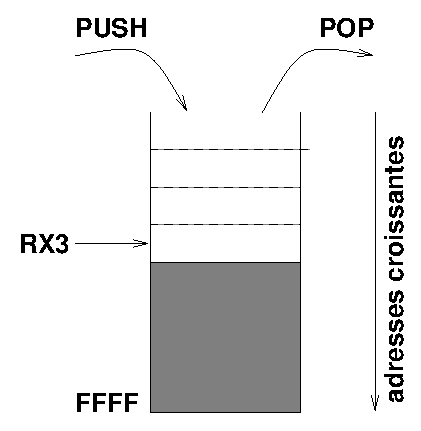
\includegraphics{pile} \\
    \end{tabular}
  \end{center}
\end{frame}
%------------------------------------------------------------------------------
\begin{frame}
  \section{Repr\'esentation des variables locales~: le code assembleur}%
  Les variables locales \`a une fonction sont stock\'ees dans la pile.
  \par\smallskip
  Le registre \%EBP (Base Pointer) contient un d\'eplacement
  correspondant \`a une position dans la pile.
  \par\smallskip
  Il sert \`a pointer sur une donn\'ee dans la pile. 

        Repr\'esentation d'une variable locale dans la pile~:
\begin{verbatim}
int globale = 7 ;           .globl globale .data                 
                            globale: .long   7                   
int main(void){                      .text                        
                            .globl main .type   main,@function   
    int locale = 1 ;        main:                                
    return 0 ;                      ....                         
}                                   movl    %esp, %ebp           
                                    subl    $8, %esp  
                                    .... 
                                    movl    $1, -4(%ebp)         
                                    ....                         
\end{verbatim}
\end{frame}
%------------------------------------------------------------------------------
\begin{frame}
  \section{Repr\'esentation des variables locales~: ce qui se passe sur la pile}%
  \begin{center}
      \begin{tabular}{clc}
        \verb?movl %esp, %ebp? & 
     \verb?subl $8, %esp?& 
    \verb?movl    $1, -4(%ebp)? \\
%     & \verb?andl $-16, %esp? &\\ 
    \begin{tabular}[b]{c|c|}
      \hline
      \%ESP & data   \\\hline
      & $4$ octets  \\\hline
      & $\cdots$   \\
      & $\cdots$   \\
      \hline
      FFFF & bas de pile \\\hline
    \end{tabular} &
    \begin{tabular}[b]{c|c|}
      \hline
      \%ESP & vide   \\\hline
      & vide   \\\hline
      \%EBP & data   \\\hline
      & $4$ octets  \\\hline
      & $\cdots$   \\
      & $\cdots$   \\
      \hline
      FFFF & bas de pile \\\hline
    \end{tabular} &
    \begin{tabular}[b]{c|c|}
      \hline
      \%ESP & vide   \\\hline
      & $1$        \\\hline
      \%EBP & data   \\\hline
      & $4$ octets  \\\hline
      & $\cdots$   \\
      & $\cdots$   \\
      \hline
      FFFF & bas de pile \\\hline
    \end{tabular} \\
        \%EBP mis en place &
        r\'eserver de l'espace &
        affecter la variable
  \end{tabular}
  \end{center}
\end{frame}
%------------------------------------------------------------------------------
\begin{frame}
  \section{Repr\'esentation de variables de types diff\'erents et manipulation}%
        Peu importe le type des variables locales que l'on veut repr\'esenter,
        la m\'ethode est la m\^eme~:
        \par\bigskip
\begin{verbatim}
int main(void){                    .text                           
                       .     globl main                    
  struct Gauss{                    .type        main, @function    
    int re ;                  main:                                
    int im ;                        ....                           
  } var = {                         movl    %esp, %ebp     
    .re = 1 ,                       subl    $24, %esp      
    .im = 1 ,                       ....                           
  } ;                               movl        $1, -8(%ebp)       
                                    movl        $1, -4(%ebp)
  char tab[2] = {'a','b'} ;         movb    $97, -10(%ebp)
                                    movb    $98, -9(%ebp)
  tab[0] += tab[1] ;                movb    -9(%ebp), %dl
                                    leal    -10(%ebp), %eax
                                    addb    %dl, (%eax)
  return 0 ; }                      ....                       
\end{verbatim}
\end{frame}
%------------------------------------------------------------------------------
\begin{frame}
  \section{Rappel sur les registres associ\'es \`a l'ex\'ecution du code}%

        Le code ex\'ecutable d'un programme se pr\'esente sous la forme 
        d'une suite finie contig\"ue d'octets stock\'ee dans un segment 
        de la m\'emoire.

        \paragraph{Le registre \%CS (Code Segment).} Ce registre~$16$
        bits contient le num\'ero du segment m\'emoire dans lequel
        sont stock\'e les instructions assembleur du code \`a
        ex\'ecuter.  On ne peut pas acc\'eder directement \`a ce
        registre.

        \paragraph{Le registre \%EIP (Instruction Pointer).}  Le
        registre \%eip contient l'offset de la procha\^\i{}ne
        instruction \`a ex\'ecuter.  Il est modifi\'e automatique \`a
        chaque ex\'ecution et peut \^etre manipul\'e par des
        instruction du type \texttt{jmp}, \texttt{call}, \texttt{ret},
        etc. On ne peut pas acc\'eder directement \`a ce registre.
\end{frame}
%------------------------------------------------------------------------------
\begin{frame}
  \section{Les instructions assembleur \texttt{call} et
  \texttt{ret}}%

        L'appel d'un ``sous-programme'' se fait par %
        \verb+call label_du_sous-programme+. 
        Soit un code implant\'e \`a l'adresse
        1000 et une proc\'edure \`a l'adresse 1100.

\begin{verbatim}
  1000 mov $1,%eax             |---> label: 1100 shl $1,%eax    
  1002 mov $3,%ebx             |            1102 add %ebx,%eax    
  1004 CALL label  ------------|            1104 and $7,%eax     
  1007 mov $2,%eax <-----------|            1106 add '0',%eax   
  1009 int 0x80                |-----       1108 RET          
\end{verbatim}
        
Le sous-programme doit contenir l'instruction RET qui permet de revenir au
programme appelant. 


Lors du CALL, \%eip re\c{c}oit la valeur 1100, adresse de la prochaine
instruction \`a ex\'ecuter, tandis que l'adresse de retour 1007 est
empil\'ee sur la pile.

Sur le RET, le sommet de pile de valeur 1007 est d\'epil\'e, et son
contenu est rang\'e dans \%eip.
\end{frame}
%------------------------------------------------------------------------------
\begin{frame}
  \section{Appel de fonction en~C (sans param\`etre)}%
        \begin{verbatim}
int UN(void){                           .text                        
        return 1 ;             .globl UN                        
}                               UN:                                
                                       ...                        
int main(void){                        movl    $1, %eax        
                                       ...                        
        int var = UN() ;               ret                       
        return 0 ;                     
}                               .globl main                        
                               main:                                
/* Remarquez que la valeur             ...                        
   de retour transite par              movl    %esp, %ebp        
   le registre %eax        */          subl    $8, %esp        
                                       ....                        
                                       call    UN                
                                       movl    %eax, -4(%ebp)        
                                       movl    $0, %eax        
                                       ...                        
                                       ret                        
                                       ...                     
\end{verbatim}
\end{frame}
%------------------------------------------------------------------------------
\begin{frame}
  \section{Ce qui se passe sur la pile}%
  \begin{center}
      \begin{tabular}{ccc}
     \begin{tabular}[b]{c|c|}
      \hline
      \%ESP & vide   \\\hline
      & var.\ local        \\\hline
      \%EBP & data   \\\hline
      & $4$ octets  \\
      \hline
      FFFF & bas de pile \\\hline
    \end{tabular} &
     \begin{tabular}[b]{c|c|}
      \hline
      \%ESP & adresse  \\
 & de retour   \\\hline
          & vide   \\\hline
      & var.\ local \\\hline
      \%EBP & data   \\\hline
      & $4$ octets  \\
      \hline
      FFFF & bas de pile \\\hline
    \end{tabular} &
     \begin{tabular}[b]{c|c|}
      \hline
      \%ESP & vide   \\\hline
      & var.\ local        \\\hline
      \%EBP & data   \\\hline
      & $4$ octets  \\
      \hline
      FFFF & bas de pile \\\hline
    \end{tabular} 
         \\
        avant le call & pendant le call & apr\`es le ret 
  \end{tabular}
  \end{center}
\end{frame}
%------------------------------------------------------------------------------
\begin{frame}
  \section{Passage de param\`etres par la pile}%
        Comme les variables locales, les param\`etres sont stock\'es
        dans la pile. Dans une fonction~C les variables et 
        les param\`etres sont g\'er\'es en suivant les \'etapes~:
        \begin{enumerate}
        \item Sauver le pointeur de base de pile courant sur la pile~;
        \item Se donner un nouveau pointeur de base de pile~;
        \item Laisser de la place sur la pile les variables locales~;
        \item[] En cas d'appel de fonction avec passage de param\`etres~:
        \item Empiler les param\`etres sur la pile~;
        \item Effectuer un \texttt{call} (qui empile automatiquement
        l'adresse de retour sur la pile)~;
        \item[] Dans la fonction appel\'ee, on peut utiliser l'espace
        de pile associ\'ee aux param\`etres~;
         Cette fonction se termine par un \texttt{ret} (qui  
        d\'epile automatiquement l'adresse de retour)~;
        \item Suprimer l'espace de pile --- maintenant inutile --- 
        associ\'e aux param\`etres.
        \end{enumerate}
\newpage        
\begin{verbatim}
int PlusUn(int par){                      .text .globl PlusUn
                                     PlusUn:                                
        return par+1 ;                       pushl   %ebp                
}                                            movl    %esp, %ebp        
                                             movl    8(%ebp), %eax        
int main(void){                              incl    %eax                
                                             leave ret                        
        int var = 7 ;                     .globl main                        
                                     main:                                
        return PlusUn(var) ;                 pushl   %ebp                
}                                            movl    %esp, %ebp        
                                             subl    $8, %esp        
                                             movl    $7, -4(%ebp)        
                                             subl    $12, %esp        
                                             pushl   -4(%ebp)        
                                             call    PlusUn                
                                             addl    $16, %esp        
                                             leave
                                             ret                     
\end{verbatim}
\end{frame}
%------------------------------------------------------------------------------
\begin{frame}
  \section{Ce qui se passe sur la pile}%
  \begin{center}
      \begin{tabular}{ccc}
     \begin{tabular}[b]{c|c|}
      \hline
      \%ESP & adresse  \\
 & de retour   \\\hline
      & $4$ octets  \\
      \hline
      FFFF & bas de pile \\\hline
    \end{tabular} &
     \begin{tabular}[b]{c|c|}
      \hline
\%ESP & \%EBP\_old   \\\hline
       & adresse  \\
         & de retour   \\\hline
      & $4$ octets  \\
      \hline
      FFFF & bas de pile \\\hline
    \end{tabular} &
     \begin{tabular}[b]{c|c|}
      \hline
\%ESP   & \\
$\downarrow$     & \%EBP\_old   \\
\%EBP1 & \\
\hline
       & adresse  \\
         & de retour   \\\hline
      & $4$ octets  \\
      \hline
      FFFF & bas de pile \\\hline
    \end{tabular}
         \\
        d\'ebut de fonction & empilement de l'ancien & 
        placement du nouveau\\
        & pointeur de base  & pointeur de base
  \end{tabular}
  \end{center}
\end{frame}
%------------------------------------------------------------------------------
\begin{frame}
  \section{Ce qui se passe sur la pile}%
  \begin{center}
      \begin{tabular}{ccc}
     \begin{tabular}[b]{c|c|}
      \hline
\%ESP &    \\\hline
      & var.\ loc.\   \\\hline
\%EBP1 & \%EBP\_old   \\\hline
       & adresse  \\
         & de retour   \\\hline
      & $4$ octets  \\
      \hline
      FFFF & bas de pile \\\hline
    \end{tabular} &
     \begin{tabular}[b]{c|c|}
      \hline
\%ESP & param\`etres    \\\hline
      & var.\ loc.\   \\\hline
\%EBP1 & \%EBP\_old   \\\hline
       & adresse  \\
         & de retour   \\\hline
      & $4$ octets  \\
      \hline
      FFFF & bas de pile \\\hline
    \end{tabular} &
     \begin{tabular}[b]{c|c|}
      \hline
\%ESP       & adresse  \\
         & de retour   \\\hline

      & param\`etres    \\\hline
      & var.\ loc.\   \\\hline
\%EBP1 & \%EBP\_old   \\\hline
       & adresse  \\
         & de retour   \\\hline
      & $4$ octets  \\
      \hline
      FFFF & bas de pile \\\hline
    \end{tabular} 
         \\
        cr\'eation de variables & empilement de param\`etres & 
                apr\`es un \texttt{call} \\
        locales & 
  \end{tabular}
  \end{center}
\end{frame}
%------------------------------------------------------------------------------
\begin{frame}
  \section{Ce qui se passe sur la pile}%
  \begin{center}
      \begin{tabular}{ccc}
     \begin{tabular}[b]{c|c|}
      \hline
\%ESP & var.\ loc.\   \\\hline
\%EBP & \%EBP1   \\\hline
       & adresse  \\
         & de retour   \\\hline
      & param\`etres    \\\hline
      & var.\ loc.\   \\\hline
\%EBP & \%EBP\_old   \\\hline
       & adresse  \\
         & de retour   \\\hline
      & $\vdots$\\
        \hline
    \end{tabular} &
        \begin{minipage}[b]{7cm}
        \`A la fin de la nouvelle fonction
        \begin{itemize}
        \item une instruction \texttt{leave} permet d'enlever de la
        pile l'espace associ\'e aux variables locales et au stockage
        du pointeur de base. De plus, elle r\'eaffecte au registre
        \%EBP la valeur du pointeur de base de la fonction appelante~;
        \item l'instruction \texttt{ret} d\'epile l'adresse de retour et
        positionne le registre pointeur d'instruction \`a cette adresse.
        \item il ne reste plus qu'\`a supprimer de la
        pile l'espace associ\'e aux param\`etres (\verb?addl $16,%esp?)
        pour se retrouver dans la situation d'avant l'appel de fonction.
        \end{itemize}
        \end{minipage}
         \\
        dans la nouvelle fonction
  \end{tabular}
  \end{center}
\end{frame}
%------------------------------------------------------------------------------
\begin{frame}
  \section{Passage de param\`etre par copie~: une copie est faite sur la pile}%
\begin{verbatim}
                                   .text                                         
                                 .globl PER            .globl main   
                                PER:                    main:         
void PER(int alpha, int beta){    pushl %ebp               pushl %ebp     
       int tmp = alpha ;          movl  %esp, %ebp         movl  %esp, %ebp    
       alpha = beta ;             subl  $4, %esp           subl  $8, %esp  
       beta = alpha ;             movl  8(%ebp), %eax      andl  $-16, %esp    
}                                 movl  %eax, -4(%ebp)     movl  $1, -4(%ebp)  
                                  movl  12(%ebp), %eax     movl  $1, -8(%ebp)  
int main(void){                   movl  %eax, 8(%ebp)      subl  $8, %esp  
                                  movl  8(%ebp), %eax      pushl -8(%ebp)  
        int a = 1 ;               movl  %eax, 12(%ebp)     pushl -4(%ebp)  
        int b = 1 ;               leave                    call  PER       
        PER(a,b) ;                ret                      addl  $16, %esp 
        return 0 ;                                         movl  $0, %eax  
}                                                          leave           
                                                           ret            
\end{verbatim}
\end{frame}
%------------------------------------------------------------------------------
\begin{frame}
  \section{Passage de param\`etre par adresse~: les adresses sont copi\'ees sur la pile}%
\begin{verbatim}
                                          .text                   
                                  .globl PER                   .globl main                
                                  PER:                   main:                        
void PER(int *alpha, int *beta){    pushl %ebp              pushl %ebp                
       int tmp = *alpha ;           movl  %esp, %ebp        movl  %esp, %ebp        
       *alpha = *beta ;             subl  $4, %esp          subl  $8, %esp        
       *beta = *alpha ;             movl  8(%ebp), %eax     andl  $-16, %esp        
}                                   movl  (%eax), %eax      movl  $1, -4(%ebp)        
                                    movl  %eax, -4(%ebp)    movl  $1, -8(%ebp)        
int main(void){                     movl  8(%ebp), %edx     subl  $8, %esp        
                                    movl  12(%ebp), %eax    leal  -8(%ebp), %eax  
        int a = 1 ;                 movl  (%eax), %eax      pushl %eax                
        int b = 1 ;                 movl  %eax, (%edx)      leal  -4(%ebp), %eax  
        PER(&a,&b) ;                movl  12(%ebp), %edx    pushl %eax                
        return 0;                   movl  8(%ebp), %eax     call  PER                
}                                   movl  (%eax), %eax      addl  $16, %esp        
                                    movl  %eax, (%edx)      movl  $0, %eax        
                                    leave                   leave                              
                                    ret                     ret              
\end{verbatim}
\end{frame}
%------------------------------------------------------------------------------
\begin{frame}
  \section{Passage de param\`etre de type structure}%
\begin{verbatim}
typedef  struct Gauss_t{              .text                      .globl main   
    int re ;                    .globl UN               main:             
    int im ;                UN:                              pushl   %ebp    
  } Gauss_t ;                   pushl %ebp                   movl  %esp, %ebp  
                                movl  %esp, %ebp             subl  $8, %esp    
void UN(Gauss_t par){           subl  $8, %esp               andl  $-16, %esp  
   par.re = 2 ;                 movl  8(%ebp), %eax          movl  $1,-8(%ebp) 
}                               movl  12(%ebp), %edx         movl  $1,-4(%ebp) 
                                movl  %eax, -8(%ebp)         subl  $8, %esp   
int main(void){                 movl  %edx, -4(%ebp)         pushl -4(%ebp)    
                                movl  $2, -8(%ebp)           pushl -8(%ebp)    
   struct Gauss_t var ;         leave                        call  UN      
   var.re = 1 ;                 ret                          addl  $16,
   var.im = 1 ;                                              movl  $0, %eax   
                                                             leave         
   UN(var) ;                                                 ret             

   return 0 ;
}                         
\end{verbatim}
\end{frame}
%------------------------------------------------------------------------------
\begin{frame}
  \section{Passage de param\`etre de type structure avec structure retourn\'ee}%
\begin{verbatim}
typedef  struct Gauss_t{                   .text                 
    int re ;                          .globl UN                      .globl main   
    int im ;                     UN:                          main:           
  } Gauss_t ;                       pushl %ebp               pushl %ebp            
                                    movl  %esp, %ebp         movl  %esp, %ebp  
struct Gauss_t UN(Gauss_t par){     subl  $8, %esp           subl  $24, %esp   
   par.re = 2 ;                     movl  8(%ebp), %eax      andl  $-16, %esp  
   return par ;                     movl  12(%ebp), %edx     movl  $1, -8(%ebp)
}                                   movl  16(%ebp), %ecx     movl  $1, -4(%ebp)
                                    movl  %edx, -8(%ebp)     leal  -16(%ebp),%eax       
int main(void){                     movl  %ecx, -4(%ebp)     subl  $4, %esp    
                                    movl  $2, -8(%ebp)       pushl -4(%ebp)    
   struct Gauss_t var,res ;         movl  -8(%ebp), %edx     pushl -8(%ebp)    
   var.re = 1 ;                     movl  -4(%ebp), %ecx     pushl %eax               
   var.im = 1 ;                     movl  %edx, (%eax)       call  UN                                            
                                    movl  %ecx, 4(%eax)      addl  $12, %esp   
   res = UN(var) ;                  leave                    movl -16(%ebp),%eax
   var.im = res.re ;                ret   $4                 movl %eax,-4(%ebp)
   return 0 ;                                                movl  $0,%eax
}                                                            leave ret
 \end{verbatim}
\end{frame}
%------------------------------------------------------------------------------
\end{document}
%------------------------------------------------------------------------------
%------------------------------------------------------------------------------
\begin{frame}
  \section{}%
\end{frame}
%------------------------------------------------------------------------------
